\documentclass[a4paper,10pt]{article}

\usepackage[latin1]{inputenc}
\usepackage{amsfonts}
\usepackage{amsmath}
\usepackage{amssymb}
\usepackage{amsthm}
\usepackage[ngerman]{babel}
\usepackage[T1]{fontenc}
\usepackage[dvips,pdftex]{graphicx}
\usepackage{pst-all}
\usepackage{xcolor}

\usepackage[dvips]{hyperref}


\author{Klasse 2B}
\title{�bungsblatt Lineare Funktionen}
\date{Schuljahr 2007-2008}

\begin{document}
\maketitle

\begin{enumerate}
\item Wie lautet die Gleichung der Geraden, die durch $P(-1|2)$ geht und
zu der Geraden durch $A(0|-1)$ und $B(3|3)$ parallel ist?

\hfill (L�sung: $y={\frac43}x + {\frac{10}{3}}$)

\item 
Die Punkte $A(2|3)$ und $B(7|7)$ bestimmen den Graphen einer
linearen Funktion $g$.
\begin{enumerate}
\item
Bestimme den Funktionsterm $g(x)$.
\item
Gib den Funktionsterm einer linearen Funktion $f$ an, deren
Graph parallel zu dem von $g$ verl"auft und durch den 
Punkt $R(5|2)$ geht. 
\end{enumerate}


\hfill (L�sung:$g(x)={\frac45} x+ {\frac75}$, $f(x)={\frac45} x-2$)


\item Wie lautet die Funktionsgleichung der Parallelen zu 
$y=\frac{7}{3}x-\frac{12}{5}$ durch den Punkt\\
$P(18|-23)$?

\hfill (L�sung: $y=\frac{7}{3} x - 65$)



\item Gegeben ist die Funktion $f: \;x \longmapsto -2x - 3$.
\begin{enumerate}
\item
  Begr"unde ohne Zeichnung, in welchen Quadranten der Graph der Funktion
  verl"auft.
\item
  Bestimme die Schnittpunkte mit den Koordinatenachsen und zeichne
  den Graphen.
\item
  Zeige durch Rechnung, dass der Punkt P$(3|-9)$ auf dem Graphen,
  der Punkt Q$(-12|-13)$ jedoch nicht auf dem Graphen liegt.
\item
  Wie lautet die Funktionsvorschrift derjenigen linearen Funktion,
  auf deren Graphen sowohl $P$ als auch $Q$ liegt.
\end{enumerate}
%

\hfill (L�sung:(b) $x=-1{,}5;\; y=-3\quad$ (d) $y= \frac{4}{15}x - 9{,}8$)



\item Durch die folgenden Gleichungen sind zwei Geraden gegeben:
$$
(1) \ \ y={\frac23}x + 1,5 \hskip 2 cm  (2) \ \ 0=2y-3x+4,5
$$
Zeichne ihre Graphen und bestimme graphisch die L"osung des
Gleichungssystems.

\hfill  (L�sung:$(4,5|4,5)$)



\item \begin{enumerate}
\item
Berechne die Nullstelle der Funktion $h: x \longmapsto {\frac35} x-2$.
\item
Der Graph $G_g$ einer Funktion $g$ verl"auft durch den Punkt $P(3|2)$
und ist parallel zum Graphen $G_h$ der Funktion $h$. Gib den Funktionsterm 
der Funktion $g$ an. 
\end{enumerate}

\hfill (L�sung:(a) Nullstelle $x={\frac{10}{3}}$, (b) Funktionsterm $g(x)={\frac35}x +{\frac15}$.)




\item Die Punkte $A(-1|6)$ und $B(6|3)$ sind Elemente der Geraden $g$. Die 
Gerade $h$ geht durch den Punkt $C(1|2)$ und hat die Steigung $\frac{3}{4}$. 
\begin{enumerate}
\item Ermittle graphisch die Koordinaten des Schnittpunktes $S$ von 
$g$ und $h$!
\item Stelle die Gleichungen von $g$ und $h$ auf und berechne die 
Koordinaten von $S$!
\end{enumerate}


\hfill (L�sung: $g(x)=-\frac{3}{7}\,x+\frac{39}{7}$\quad;\quad
$h(x)=\frac{3}{4}\,x+\frac{5}{4}$\quad;\quad $S(\frac{11}{3}|4)$)


\item \begin{enumerate}
\item Zeige, dass der Punkt $P(1|3)$ auf der Geraden mit der
Gleichung \mbox{$y=-2x+5$} liegt.
\item Gib die Gleichung irgendeiner weiteren Geraden an, auf
welcher der Punkt $P(1|3)$ liegt.
\end{enumerate}



\hfill \begin{enumerate}
\item (L�sung:$-2\cdot 1+5=3 \Rightarrow$ $P$ liegt auf der Gerade
\hfill \item Z.\ B.\ $y=-3x+6$)
\end{enumerate}

\item Gegeben ist die Funktion $f: \;x \longmapsto -2x - 3$.
\begin{enumerate}
\item
  Begr"unde ohne Zeichnung, in welchen Quadranten der Graph der Funktion
  verl"auft.
\item
  Bestimme die Schnittpunkte mit den Koordinatenachsen und zeichne
  den Graphen.
\item
  Zeige durch Rechnung, dass der Punkt P$(3|-9)$ auf dem Graphen,
  der Punkt Q$(-12|-13)$ jedoch nicht auf dem Graphen liegt.
\item
  Wie lautet die Funktionsvorschrift derjenigen linearen Funktion,
  auf deren Graphen sowohl $P$ als auch $Q$ liegt.
\end{enumerate}
%

\hfill  (L�sung:(b) $x=-1{,}5;\; y=-3\quad$ (d) $y= \frac{4}{15}x - 9{,}8$)





\item Weise durch  Rechnung nach, dass die Punkte
$A(-5|\frac{35}{4})$, $B(4|2)$ und $C(7|-\frac{1}{4})$
auf einer Geraden liegen.

\hfill  (L�sung:Die Steigungen der beiden Geraden $AB$ und $AC$ stimmen "uberein
($m=-0{,}75$).)






\item In einem Koordinatensystem (L"angeneinheit 1\,cm) sind die Punkte
$A(7|0)$ und $B(5|4)$ sowie die Gerade $g_1$ durch die Gleichung
$3x-4y+12=0$ gegeben.
\begin{enumerate}
\item	Zeichne die Punkte $A$ und $B$ sowie (mit Hilfe eines
	Steigungsdreiecks) die Gerade $g_1$ in das Koordinatensystem ein!
\item	Die Gerade $g_1$ schneidet die y-Achse im Punkt $C$ und die 
	x-Achse im Punkt $D$. Berechne die Koordinaten von $C$ und $D$!
\item	Ermittle eine Gleichung der durch die Punkte $A$ und $B$
	bestimmten Geraden $g_2$ in expliziter Form!
\item	Berechne ausf"uhrlich den Inhalt des Vierecks $ABCD$!
\end{enumerate}



\hfill  (L�sung:(b):~~$C(0|3),~D(-4|0)$;~~(c):~$y=-2x+14$;~~
	(d):~$A_{ABCD}=27,5\,cm^2$)






\item In einer Badewanne befinden sich 105 Liter Wasser. Nachdem der St"opsel
herausgezogen wurde, flie"sen pro Minute 18 Liter Wasser durch den Ausgu"s ab.
\begin{enumerate}
\item
Zeichne den Graphen der Zuordnung Zeit $\mapsto$ Wassermenge in der Wanne.
\item
Gib die Zuordnungsvorschrift an.
\item
Berechne die Zeitdauer in Minuten und Sekunden, bis die Wanne leer ist.
\end{enumerate}


\hfill  (L�sung:b) x: Zeit in Minuten; y:Wassermenge in Litern; $y=105 - 18x$\\
c) $5\,$min $50\,$s)


\item {\tiny .}
%\begin{minipage}[t]{8cm}
Gib die Funktionsgleichungen der Geraden $g$ und $h$ an und
berechne die Koordinaten ihres Schnittpunktes $S$!
%\end{minipage}
\hfill
%\begin{minipage}[t]{7cm}
\begin{center}
 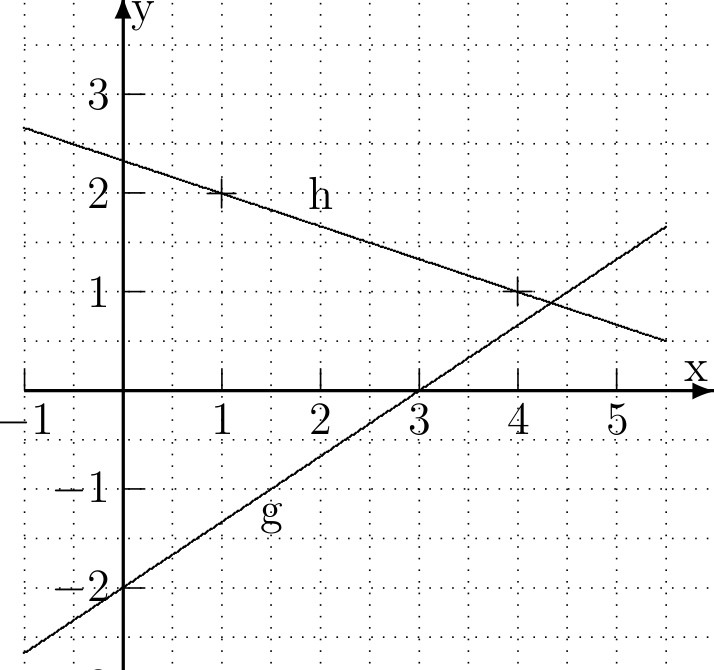
\includegraphics[width=9cm]{bilder/schnittpunkte.png}
\end{center}


%\end{minipage}


\hfill (L�sung:$g: \, y = \frac{2}{3} x - 2$;\\
\hfill $h: \, y= - \frac{1}{3} x + 2 \frac{1}{3}$;\\
\hfill  $S(4\frac{1}{3}|\frac{8}{9})$)

\end{enumerate}
\end{document}
